\section{Business Model}
\label{sec:business_model}

In this section we develop the business model of the CCaaS service offerings. To this end we mainly
use the Business Model Canvas developed by \cite{osterwalderBusinessModelGeneration2010}. Figure ...
shows a graphical summary of the business model canvas. The value proposition developed in the previous
two sections is inserted into the center of the canvas. In the following we develop the remaining building
blocks of the canvas.

\subsection{Customer Segments}

As developed in Section \ref{sec:customer_perspective}, career counseling is used by three customer archetypes:
new job market entrants, professionals in career transition, and unemployed seeking reintegration. However, the
value proposition is similar for all three types, i.e. the service offerings are the same. Therefore, we can use
a single customer segment (\textbf{counseling clients}) for all three customer archetypes.


\subsection{Channels}

Channels are the means by which the clients access the career counseling service offerings from LinkedIn.
As LinkedIn will be the provider of CCaaS services, most channels will be operated by the intermediaries,
i.e., counselors and counseling companies.

\begin{itemize}
    \item \textbf{Web}: the CCaaS platform may be used to provide web services to customers.
            For example, a career counseling company may provide a web portal to its customers
            that uses the CCaaS API layer to retrieve job recommendations and career advice for
            the customer. Also, LinkedIn can offer its own platform for users to find career
            counselors based on geographic location, expertise, etc.
    \item \textbf{Mobile}: the CCaaS platform may be used to provide mobile services to customers.
            For example, a career counseling company may provide a mobile app to its customers
            that uses the CCaaS API layer to retrieve job recommendations and career advice for
            the customer.
\end{itemize}

\subsection{Customer Relationships}

Customer relationships are the types of relationships that LinkedIn establishes with the career
counseling clients. Based on the platform argument introduced in Section \ref{sec:customer_perspective},
the relationship may not be a direct one (i.e., between LinkedIn and the customer segment). Instead, 
the customers have a relationship with a career counselor (or a counseling company) that uses the
CCaaS API layer to render its counseling services.

\begin{itemize}
    \item \textbf{Personal assistance}: career counselors may individually follow a customer's case and 
            provide personal advice. The CCaaS platform may be used to support the career counselor
            in his/her work by providing contextual recommendations and suggestions based on the 
            current client being advised.
    \item \textbf{Automated services}: the service offerings are provided as automated services, i.e. 
            the customer can use the service without the need for (a human) personal assistance.
            A counseling company may, e.g., automate the retrieving of job recommendations and 
            career path suggestions for each client by using the CCaaS API layer and forward
            these recommendations to the client. 
\end{itemize}

\begin{landscape}
        \begin{figure}
                \centering
                \caption{Business Model Canvas for CCaaS.}
                \label{fig:bmc}
                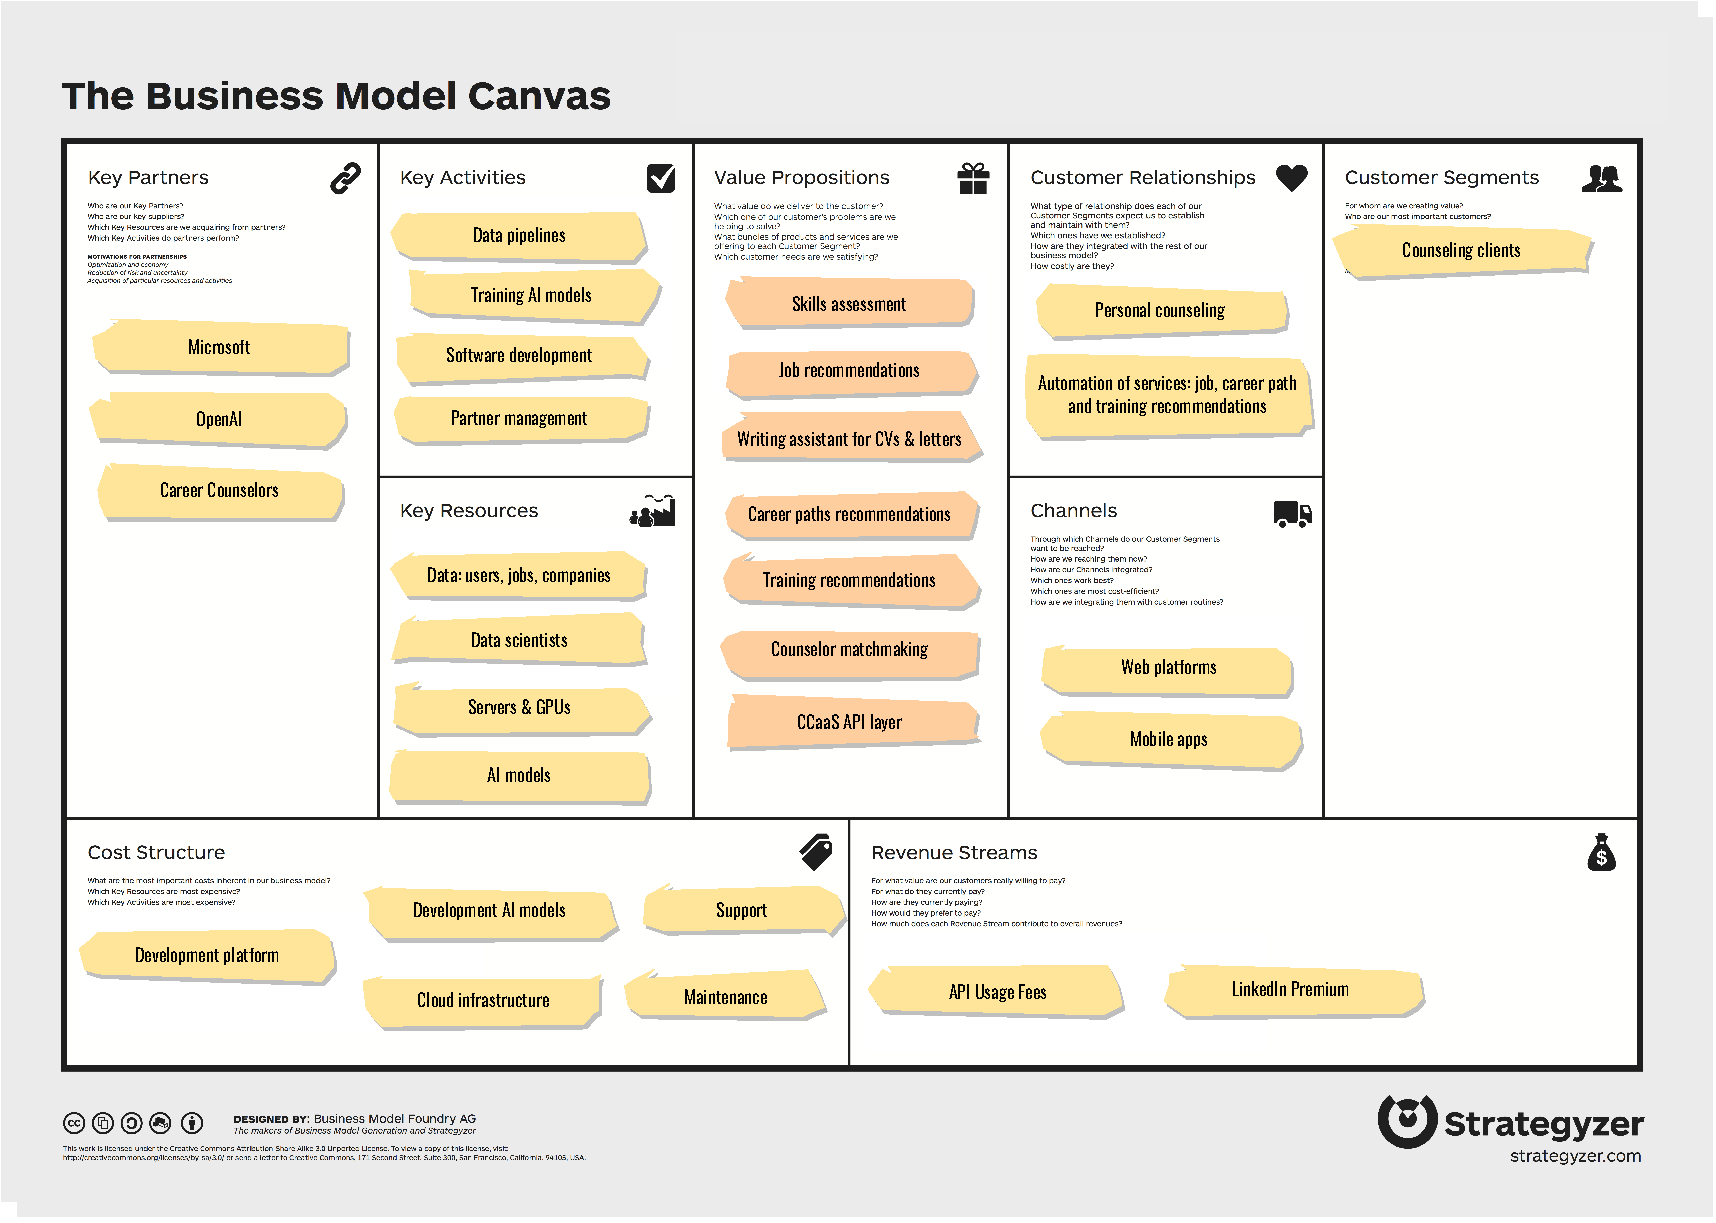
\includegraphics[width=1.3\textwidth]{figures/bmc.pdf}
        \end{figure}
\end{landscape}

\subsection{Key Activities}

Key activities represent the important things that LinkedIn must do to make the CCaaS platform work
and to offer the career counseling services via its API layer (ultimately enabling the counselors
to render the value proposition to clients).

\begin{itemize}
    \item \textbf{Data Pipelines}: LinkedIn needs to collect data from its users and store it in
            regular databases and graph databases. This activity includes designing the data model,
            architecting the data systems, developing the data pipelines, testing and deploying them,
            and monitoring and maintaining them once in production. Additionally, data pipelines for
            feedback data from career counselors and users on recommendations need to be developed.
    \item \textbf{Training AI Models}: Similarly, LinkedIn needs to train AI models and recommender
            systems on the collected data. This activity includes designing, training and evaluation
            artificial neural networks (ANN), architecting the AI systems, testing and deploying AI models,
            and monitoring and maintaining them once in production. Feedback data from career counselors
            and users on recommendations need to be used to re-train and fine-tune the AI models used 
            for recommender engines.
    \item \textbf{Software Development}: LinkedIn needs to develop the CCaaS API layer and integrate
            it into the existing LinkedIn platform and services. This activity includes designing, developing,
            testing, deploying and documenting the API layer.
    \item \textbf{Partnership Management and Support}: LinkedIn needs to manage its partnerships with
            career counseling companies and technology partners. This activity includes onboarding of
            new partners to the CCaaS platform, technical consulting regarding the integration of the 
            CCaaS API layer, and support.
\end{itemize}

\subsection{Key Resources}

Key resources describe the most important tangible assets required to make the business model work. These
assets may not be owned by LinkedIn, but may be acquired from key partners.

\begin{itemize}
        \item \textbf{Data:} First and foremost, LinkedIn's data on users, companies, and jobs is the most
                important asset for the CCaaS business model. The data is used to train effective AI models
                and recommender systems.
        \item \textbf{Data Scientists:} LinkedIn's (and by extension via Microsoft and OpenAI) data engineers 
                and data scientists are a crucial asset for the CCaaS business model. They are responsible for
                designing data models, architecting and developing data pipelines, training and evaluating
                AI models and recommender systems, and monitoring and maintaining them once in production.
        \item \textbf{Servers and GPUs:} servers and GPU's are required for intensive computational tasks 
                such as training the CCaaS AI models and recommender systems. GPU servers are also needed 
                for running the services via the API, i.e., at inference time.
        \item \textbf{AI Models:} the design and architecture of AI models (artificial neural networks) and
                recommender systems that are used to provide personalized automation in the CCaaS business model.
\end{itemize}

\subsection{Key Partnerships}

Key partnerships are not just suppliers, but real partners of the digital ecosystem in terms of value
co-creation and rendering the products and services to the end customers.

\begin{itemize}
    \item \textbf{Microsoft / OpenAI}: access to the most advanced AI technology and AI research
        from Microsoft and OpenAI. The AI models used in the CCaaS business model are co-developed
        by LinkedIn, Microsoft and OpenAI.
    \item \textbf{Career Counseling Companies}: career counseling companies are the actual customers
        paying usage fees for the CCaaS API. However, they are also the partner in terms of value 
        co-creation and delivering the value to the end customers, i.e. the clients seeking career
        advice. 
\end{itemize}

\subsection{Cost Structure}

\begin{itemize}
    \item \textbf{Development}: the initial development of the CCaaS API layer and its integration into the
            existing LinkedIn platform and services (one-time fixed cost). 
    \item \textbf{Data Science}: the development, deployment and maintenance of machine learning
        models and recommender systems used by the CCaaS platform (recurring costs, mostly salaries 
        of data scientists and MLOps engineers).
    \item \textbf{Cloud Infrastructure}: the cloud infrastructure and bandwidth / traffic costs 
        relating to the CCaaS platform (recurring, variable costs that depend on the API usage).
    \item \textbf{Support}: onboarding of career counseling companies and technology partners
        to the CCaaS platform, including technical onboarding and consulting.
    \item \textbf{Maintenance}: the maintenance of the CCaaS platform.
\end{itemize}

\subsection{Revenue Streams}

\begin{itemize}
    \item \textbf{API Usage Fees}: career counseling companies pay usage fees for the CCaaS API.
        The usage fees are based on the number of calls on the different API endpoints. The pricing
        may be varied by API endpoint type, such as the type of recommendation (e.g., retrieving
        job recommendations might be cheaper than retrieving career path suggestions).
     \item \textbf{LinkedIn Premium:} LinkedIn Premium is an existing product and represents a subscription
        tier for LinkedIn. It gives premium users  access to advanced features. LinkedIn Premium can be made
        more attractive by embedding some CCaaS offerings into the premium tier. For example, Premium
        users may get access the portal for finding a suitable career counselor. 
\end{itemize}
